\section{Anhang}
\nopagebreak
\begin{figure}
	\centering
		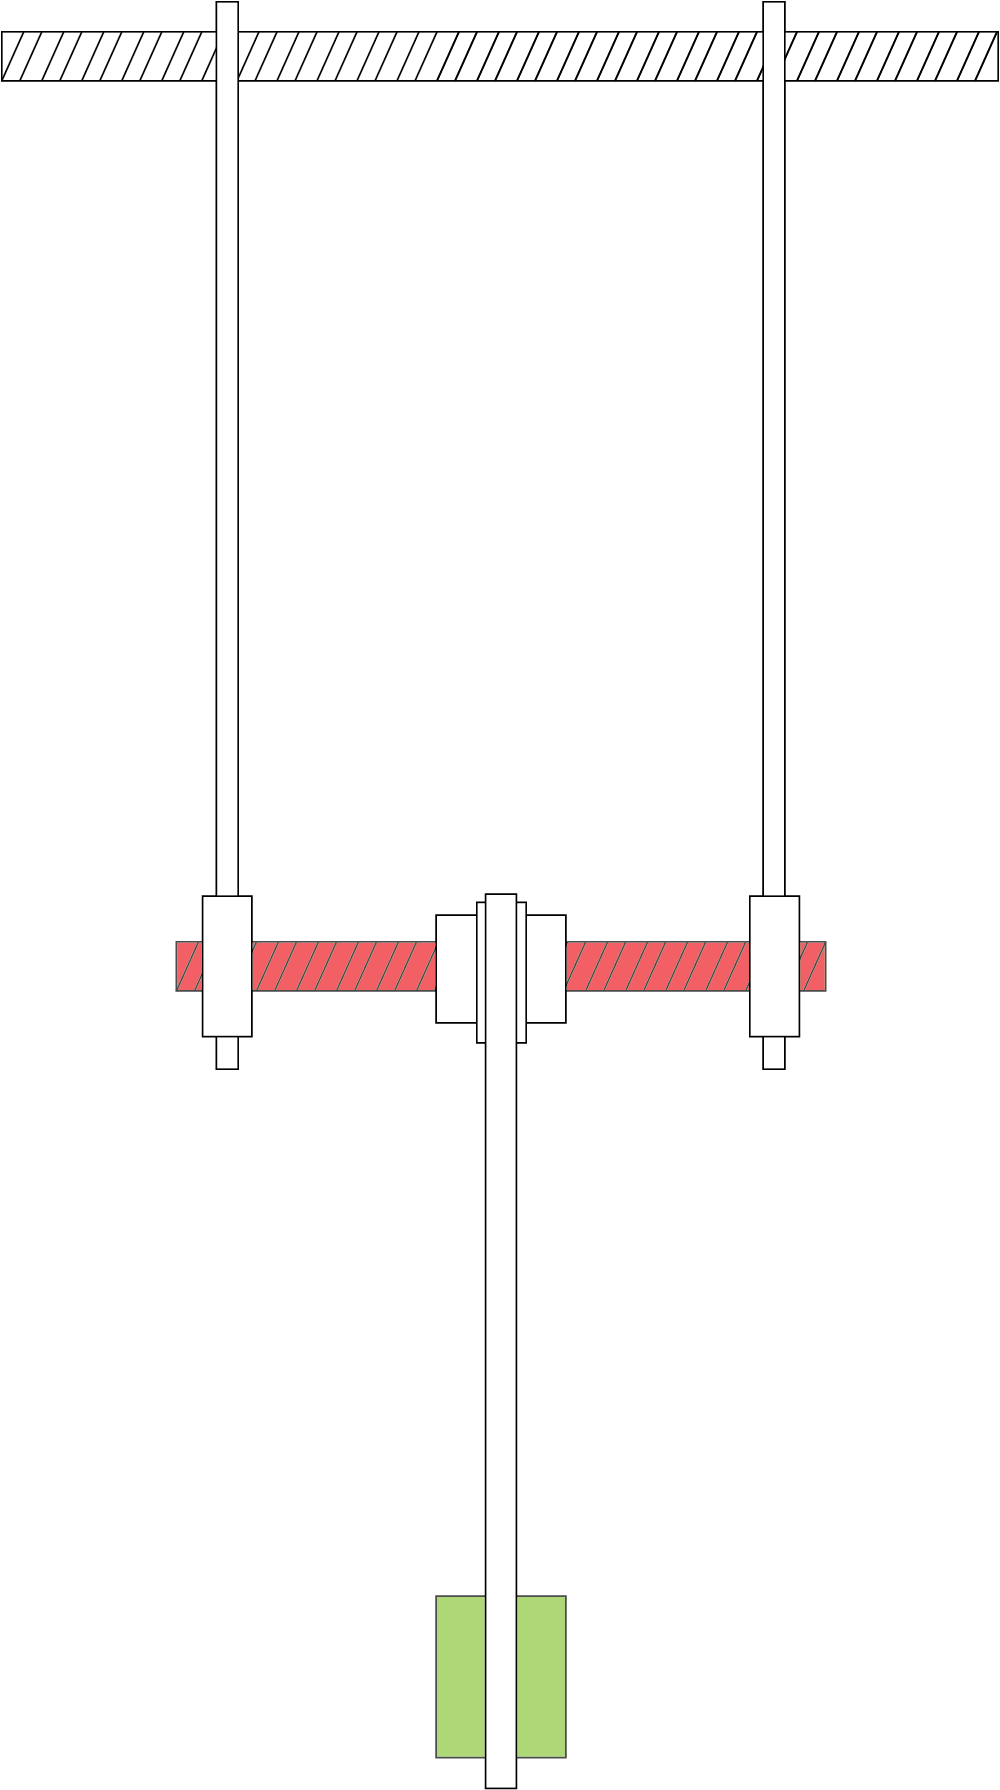
\includegraphics[width=.6\textwidth]{images/pendel-skizze.png}
	\caption{Technische Zeichnung des Pendels}
	\label{pic:skizze_versuchsaufbau}
\end{figure}
\lstset{language=Python}
\lstset{inputencoding=utf8/latin1}
\lstset{numbers=left, numberstyle=\tiny, stepnumber=2, numbersep=5pt}
\lstinputlisting[basicstyle=\footnotesize, label=code1, caption=Implementierung der Simulation in python]{sourceCode/simulation.py}

\begin{center}
\begin{longtable}{llllllllll}
\caption{Verlauf der Position der beiden Massen über die Zeit des Versuchs. Dabei wird t in s und die Position in m gemessen. (Jeder 10. Messpunkt wird dargestellt.)} \label{xy-table}\\
\hline
\textbf{t} & \textbf{x-Pos. $m_1$} & \textbf{y-Pos $m_1$} & \textbf{x-Pos. $m_2$} & \textbf{y-Pos. $m_2$} \\
\hline
\endfirsthead
\multicolumn{4}{c}%
{\tablename\ \thetable\ -- \textit{Fortsetzung}} \\
\hline
\textbf{t} & \textbf{x-Pos. $m_1$} & \textbf{y-Pos $m_1$} & \textbf{x-Pos. $m_2$} & \textbf{y-Pos. $m_2$} \\
\hline
\endhead
\hline \multicolumn{4}{r}{\textit{Fortsetzung auf der nächsten Seite}} \\
\endfoot
\hline
\endlastfoot
\input{data/tbl_v_E}
\end{longtable}
\end{center}
